\documentclass[a4paper]{article}
\usepackage[utf8]{inputenc}
\usepackage[spanish, es-tabla, es-noshorthands]{babel}
\usepackage[table,xcdraw]{xcolor}
\usepackage[a4paper, footnotesep = 1cm, width=20cm, top=2.5cm, height=25cm, textwidth=18cm, textheight=25cm]{geometry}
%\geometry{showframe}

\usepackage{tikz}
\usepackage{amsmath}
\usepackage{amsfonts}
\usepackage{amssymb}
\usepackage{float}
\usepackage{graphicx}
\usepackage{caption}
\usepackage{subcaption}
\usepackage{multicol}
\usepackage{multirow}
\setlength{\doublerulesep}{\arrayrulewidth}
\usepackage{booktabs}
\usepackage{mathrsfs,amsmath}
\usepackage{hyperref}
\hypersetup{
    colorlinks=true,
    linkcolor=blue,
    filecolor=magenta,      
    urlcolor=blue,
    citecolor=blue,    
}

\newcommand{\quotes}[1]{``#1''}
\usepackage{array}
\newcolumntype{C}[1]{>{\centering\let\newline\\\arraybackslash\hspace{0pt}}m{#1}}
\usepackage[american]{circuitikz}
\usetikzlibrary{calc}
\usepackage{fancyhdr}
\usepackage{units} 

\graphicspath{./Imagenes}

\pagestyle{fancy}
\fancyhf{}
\lhead{22.05 ASSD}
\rhead{Mechoulam, Lambertucci, Rodriguez, Londero}
\rfoot{Página \thepage}

\begin{document}
\section{Filtros}

\subsection{Introducción a filtro Anti Aliasing}
El filtro \textbf{Anti Aliasing} es un filtro pasa bajos, el cual se encarga de que se cumpla el criterio de muestreo de \textbf{Nyquist}, el cual postula  que para la reconstrucción exacta de una señal periódica continua en banda base, es necesaria una frecuencia de muestreo $f_s$  por lo menos 2 veces superior al ancho de banda B de la señal original. Bajo estas hipótesis, para reconstruir la señal solo hará falta realizar la convolución de la señal muestreada con la función sinc($B\cdot t$).
La señal original se puede expresar como:
\begin{align}
	x\left( t \right) \sim \sum_{n=-\infty}^{\infty} x\left( \frac{n}{f_s} \right) \cdot sinc \left( t-\frac{n}{f_s} \right)
\end{align}


En caso de que no se cumplan las hipótesis de Nyquist se presentará un problema el cual es facilmente observable utilizando el análisis de Fourier.
Sea x(t) una señal en tiempo continuo la cual se desea digitalizar. Utilizando un muestreo ideal, multiplicaremos la señal por un tren periódico de deltas de período $T_s = \frac{1}{f_s}$
y observaremos su transformada de Fourier.
\begin{align}
	\mathcal{F} \{x_q(t) \} (f) =\mathcal{F} \{ \delta_{T_s} (t) \cdot x(t) \} (f)=\mathcal{F} \left\lbrace \sum_{n=-\infty}^{\infty} \delta(t-nT_s) \cdot x(nT_s)\right\rbrace (f)= X(f)\  *  \ \delta_{T_S}(f)
\end{align}
\begin{align}
\delta_{T_S}(f)= \sum_{n=-\infty}^{\infty} \frac{1}{T_s} \delta(f-nf_s)
\end{align}
Dado que es sabido que el papel de la delta en una convolución es aquel de la unidad, es fácil de observar que realizar la convolución con un tren de ellas, es equivalente a montar el espectro de la señal x(t) sobre cada delta. El problema fundamental radica en la superposición de espectros entre una delta y la continua, como está ilustrado en (\ref{fig:aliassingal}) se encuentra la señal de entrada junto a su espectro , en (\ref{fig:aliasquantum}) se observa la señal cuantizada, en el caso de que se cumple el teorema de Nyquist, en cambio en (\ref{fig:alias3}) se observa el caso en el cual no se cumple el teorema, y se aprecia la superposición de espectros, en (\ref{fig:alias4}) se ve la resultante y por consiguiente en (\ref{fig:aliasfin}) la señal recuperada en caso de que no se cumpla el teorema\footnote{Las imágenes fueron extraídas de :J. G. Proakis and D. G. Manolakis, Digital signal processing. Upper Saddle River, NJ: Pearson, 2014. pag 388}.

\begin{figure}[H]
	\centering
	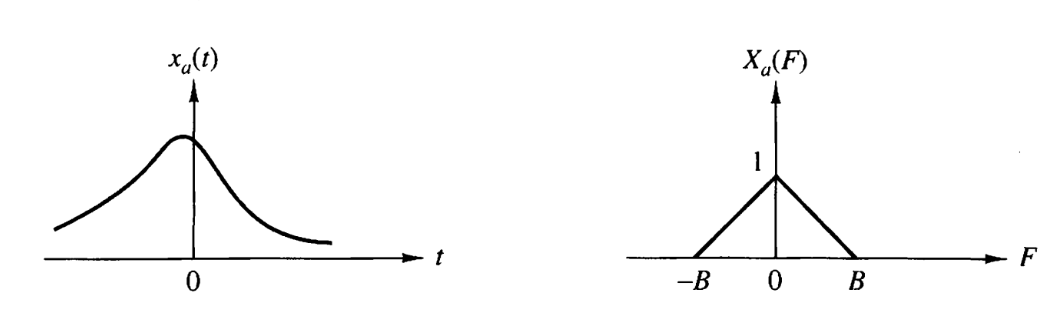
\includegraphics[width=0.8\textwidth]{ImagenesEjercicio2/aliassignal.PNG}
\caption{Señal de entrada junto a su espectro.}
	\label{fig:aliassingal}
\end{figure}

\begin{figure}[H]
	\centering
	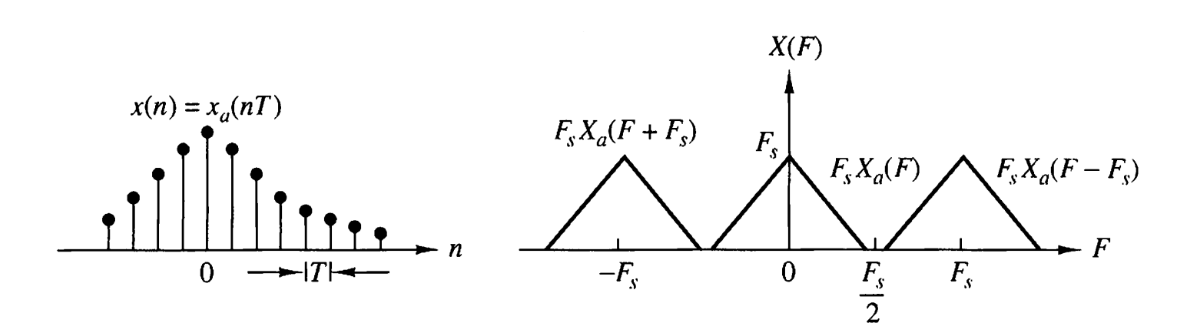
\includegraphics[width=0.8\textwidth]{ImagenesEjercicio2/aliasquatum.PNG}
\caption{Señal cuantizada junto a su espectro con $f_s > 2B$.}
	\label{fig:aliasquantum}
\end{figure}
\begin{figure}[H]
	\centering
	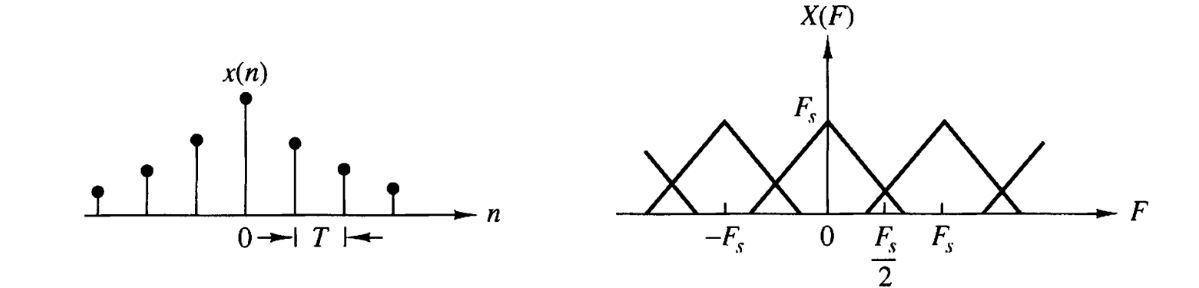
\includegraphics[width=0.8\textwidth]{ImagenesEjercicio2/alias3.PNG}
\caption{Señal cuantizada junto a su espectro con $f_s < 2B$.}
	\label{fig:alias3}
\end{figure}
\begin{figure}[H]
	\centering
	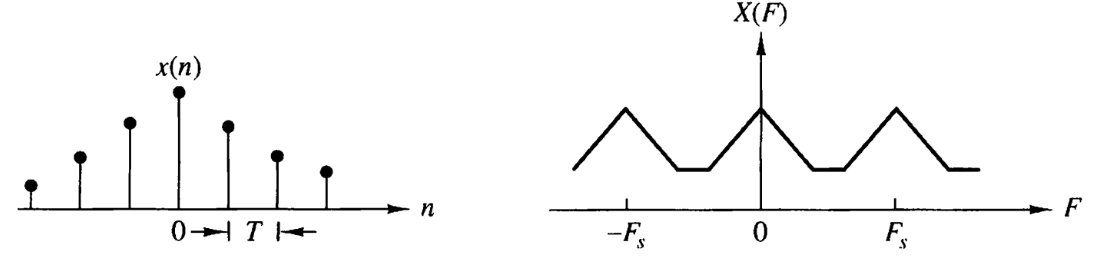
\includegraphics[width=0.8\textwidth]{ImagenesEjercicio2/alias4.PNG}
\caption{Señal cuantizada junto a su espectro resultante.}
	\label{fig:alias4}
\end{figure}
\begin{figure}[H]
	\centering
	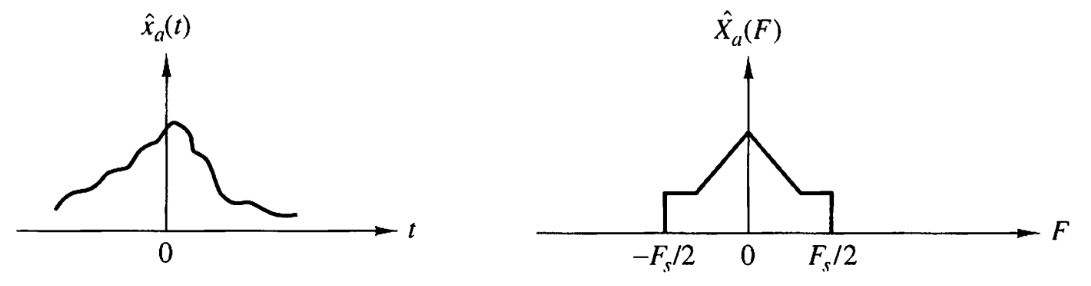
\includegraphics[width=0.8\textwidth]{ImagenesEjercicio2/aliasfin.PNG}
\caption{Señal reconstruida junto a su espectro.}
	\label{fig:aliasfin}
\end{figure}
Otro factor importante es que la frecuencia de Nyquist está definida como 2B únicamente para un filtro ideal, en la realidad se debe tomar una frecuencia mayor a $f_s>2B$ dado que se utilizará un filtro real.


%\begin{figure}[H]
%	\centering
%	\includegraphics[width=0.9\textwidth]{Ejercicio6/Imagenes/SalidaVsVLM35.png}
%\caption{Tensión de salida Vs. Tensión del LM35.}
%	\label{fig:vout}
%\end{figure}

\subsection{Introducción a filtro Recuperador}
El filtro recuperador cumple la vital importancia de como su nombre indica, recuperar la señal a partir de su espectro, dado que previo al filtro, se tiene un espectro como es observado en (\ref{fig:recuperador}) el objetivo del filtro recuperador es filtrar los espectros ajenos a la banda base, para obtener en el dominio temporal la señal original.
\begin{figure}[H]
	\centering
	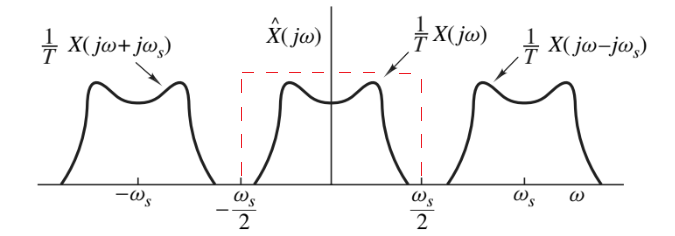
\includegraphics[width=0.8\textwidth]{ImagenesEjercicio2/recuperador.PNG}
\caption{Espectro de la señal cuantizada.}
	\label{fig:recuperador}
\end{figure}


\subsection{Análisis espectral}
En esta sección se procede a analizar el tipo de señales que recibirá el circuito, se especificaron las siguientes señales por la cátedra:
{\\\center
$X_a$ = cos(2$\pi f_{in}$ t) \ \ $\sim$  \ \
$X_b$: $\frac{3}{2}$ seno \  \ $\sim$ \ \
$X_c$ : Señal triangular \\
}
Para esto se utilizará como herramienta la serie de fourier de cada una de estas señales, con esta definida como:
\begin{align}
x(t) = \sum_{n=-\infty}^{\infty} X_n \cdot e^{j2\pi n f_0t} \ \ \ \ \wedge	\ \ \ \ X_n= \int_{-\frac{T}{2}}^\frac{T}{2} x(t) \cdot e^{-j2\pi n f_0t} dt
\end{align}
Teniendo en cuenta que tambien se puede expresar de forma trigonométrica como:
\begin{align}
x(t) = \sum_{n=0}^{\infty} a_n \cdot \cos(2\pi n f_0t) + b_n  \cdot \sin(2\pi n f_0t) \ \ \ \ \wedge	\ \ \ \ a_n = \int_{-\frac{T}{2}}^\frac{T}{2} x(t) \cdot \cos(2\pi n f_0t) dt \ \ \ \  \wedge   \ \ \ \ b_n = \int_{-\frac{T}{2}}^\frac{T}{2} x(t) \cdot \sin(2\pi n f_0t) dt 
\end{align}
Realizando las cuentas para cada señal queda que:\\



$X_a$ ya es su propio desarrollo en serie.\\ \\
\begin{align}
X_b = \sum_{n=0}^{\infty} \frac{12}{\pi} \cdot \frac{1}{9-4n^2} \cdot \cos(2\pi n f_0t) \ \ \ \ 
X_c = \sum_{n=1,3,5,...}^{\infty} \frac{8 \cdot (-1)^{\frac{n-1}{2}}}{\pi^2 n^2} \cdot \sin(2\pi n f_0t)
\end{align}
El criterio que se utilizará para saber hasta que armónico conservaremos, dado que estas ultimas 2 señales cuentan con infinitos, sera hasta obtener una potencia del 99$\%$, es útil recordar que la potencia de una señal se encuentra en sus coeficientes de fourier, mediante la \textbf{igualdad de Parseval}
\begin{align}
\frac{1}{T} \cdot \int_{-\infty}^\infty |\ x(t)\ |^2 \ =\  \sum_{n=- \infty}^{\infty} |\ X_n \ |^2
\end{align}
Para las señales $X_b$ y $X_c$ se graficó la potencia en función del armónico y como quedaría la señal reconstruida  luego de este filtro.
\begin{figure}[H]
	\centering
	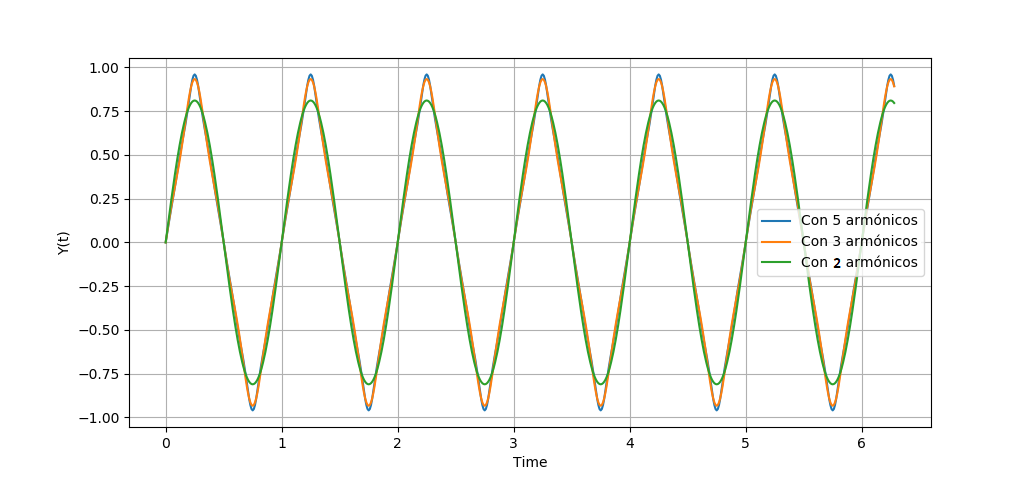
\includegraphics[width=0.85\textwidth]{ImagenesEjercicio2/10Armonicos.PNG}
	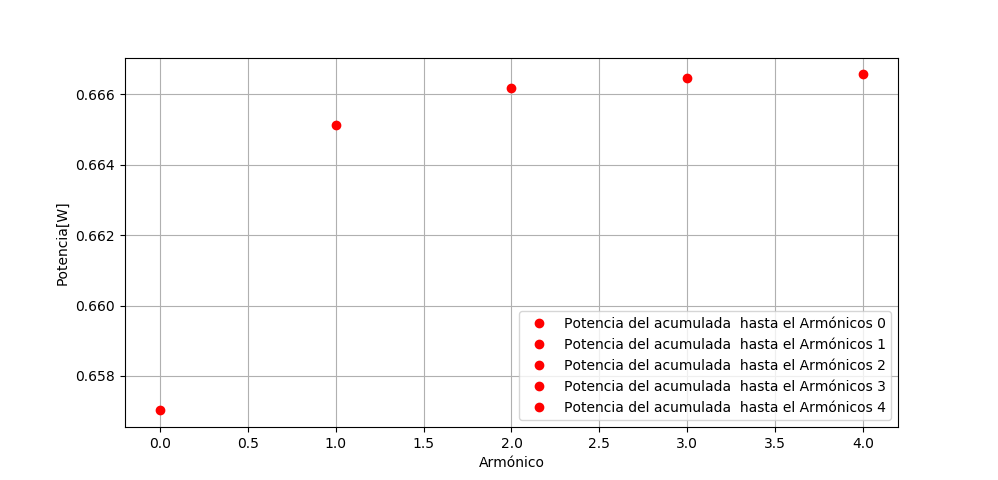
\includegraphics[width=0.85\textwidth]{ImagenesEjercicio2/4ARMONICOS.PNG}
\caption{Señal triangular reconstruida junto a su espectro de potencias.}
	\label{fig:pottriang}
\end{figure}
Es de apreciar que  tan solo con la inclusión de 2 armónicos se obtiene una potencia superior al 98$\%$\\
Luego con la señal seno $\frac{3}{2}$
\begin{figure}[H]
	\centering
	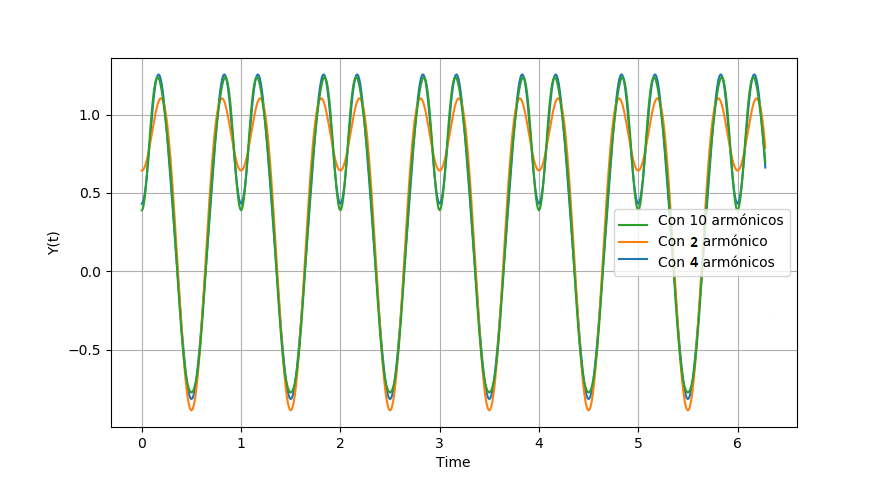
\includegraphics[width=0.85\textwidth]{ImagenesEjercicio2/sen32signal.PNG}
	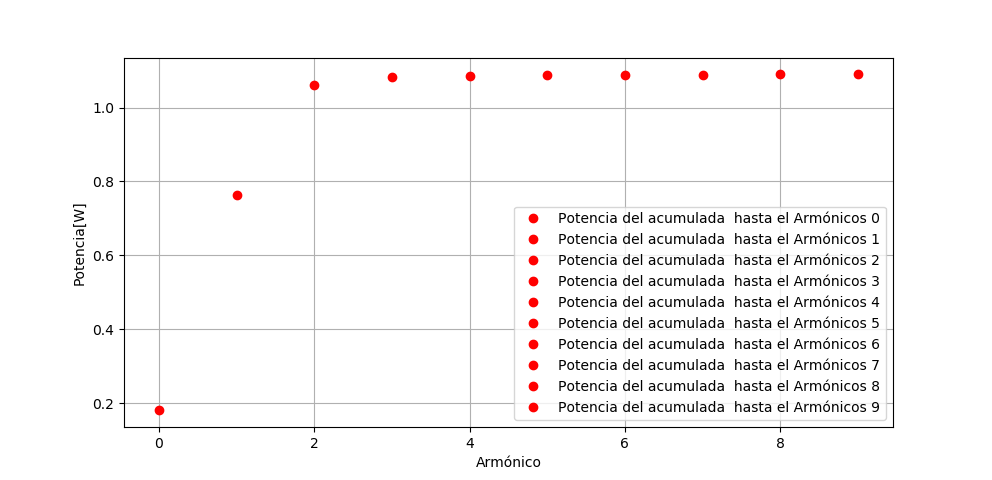
\includegraphics[width=0.85\textwidth]{ImagenesEjercicio2/sen32signalpot.PNG}
\caption{Señal seno $\frac{3}{2}$ reconstruida junto a su espectro de potencias.}
	\label{fig:potsin}
\end{figure}
Es de apreciar que  incluyendo hasta el 3er armónico se obtiene una potencia superior al 95$\%$ \\
La frecuencia fundamental de estas señales será $f_0 =\frac{N}{2} kHz = 1,5 kHz $, correspondiendole la frecuencia del máximo armónico (el 3er) de 4k5Hz, asimismo, es favorable considerar la señal de AM que también será probada por el sistema , cuya máxima frecuencia será $2,2 \cdot f_0 = 3k3Hz$. Se tomará  $f_p= 5kHz$  definiendo así la plantilla de ambos filtros.
\begin{table}[H]
\centering
\begin{tabular}{cccc}
$f_p$ & $f_a$ & $A_p$ & $A_s$ \\ \hline
5kHz & 7.5kHz & 1dB & 50dB
\end{tabular}
\end{table}
\subsection{Diseño del filtro}
 Una vez con los parámetros definidos, se procedió  a elegir la aproximación a utilizar, se descartaron cheby II y cauer, debido a los ceros de transmisión que estos poseen, y cheby 1 debido a el ripple de banda pasante que este posee, luego Guass y Bessel fueron descartados ya que su principal característica es la linealidad de la fase, finalmente quedan Butterworth y Legendre, de los cuales si bien  Butterworth tiene la mayor planicie de banda pasante , tiene el problema de que para cumplir la plantilla necesitaría un orden superior que utilizando la aproximación de legendre, ademas agrengado que legendre cuenta con el mayor cambio de pendiente, por estas razones, se eligió utilizar la aproximación de Legendre.
 Realizando la aproximación se obtuvo el siguiente diagrama de polos y ceros:
 \begin{figure}[H]
	\centering
	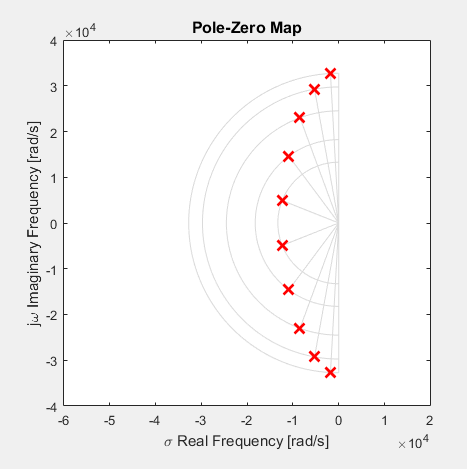
\includegraphics[width=0.65\textwidth]{ImagenesEjercicio2/polosyceros.PNG}
\caption{Diagrama de polos y ceros.}
	\label{fig:polosyceros}
\end{figure}
Ademas de obtener una transferencia teórica de la siguiente forma:
 \begin{figure}[H]
	\centering
	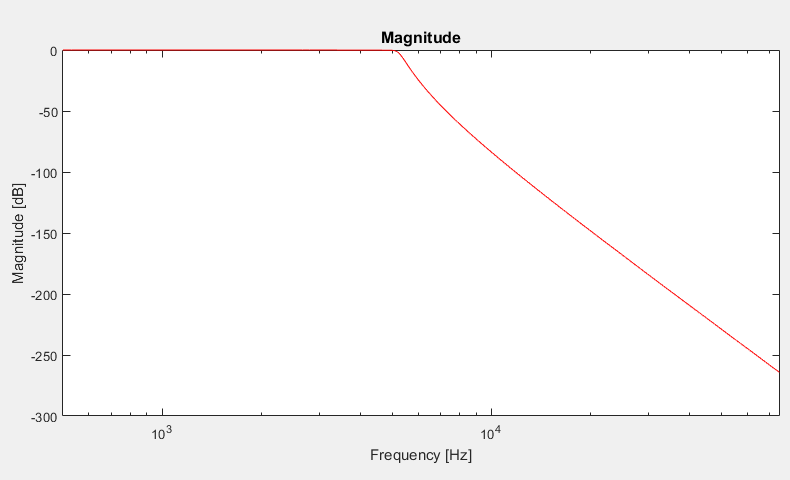
\includegraphics[width=0.8\textwidth]{ImagenesEjercicio2/atenuation.PNG}
\caption{Respuesta en frecuencia teórica.}
	\label{fig:transteorica}
\end{figure}
Lo cual corresponde a un filtro de orden 10, con frecuencias de corte y Q como indica la siguiente tabla:
\begin{table}[H]
\centering
\begin{tabular}{ccc}
\textbf{Etapa} & \textbf{Frecuencia de corte [kHz]} & \textbf{Q} \\ \hline
1 & 2.1 & 0.54 \\
2 & 2.8 & 0.84 \\
3 & 3.8 & 1.45 \\
4 & 4.6 & 2.82 \\
5 & 5.1 & 9.06
\end{tabular}
\end{table}
La topología elegida para realizar todas las  etapas fue la \textbf{Sallen Key} pasa bajos, debido a que no se alcanzan valores altos de Q
Siendo el circuito correspondiente.

\begin{figure}[H]
\centering
	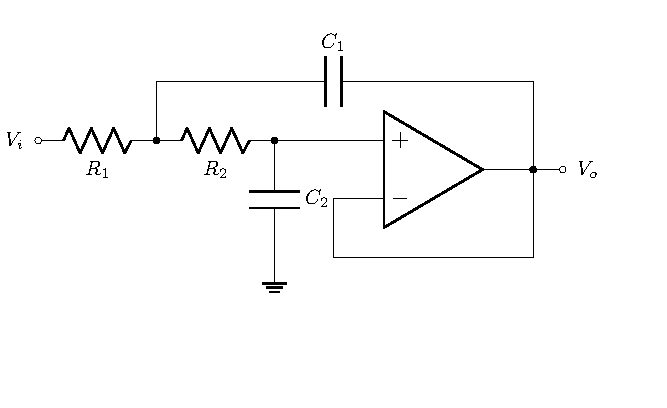
\includegraphics[width=0.9\textwidth]{ImagenesEjercicio2/SK.pdf}
	\caption{Celda Sallen Key.}
	\label{fig:SK}
\end{figure}

Luego se obtuvieron los valores para los componentes.
\begin{table}[H]
\centering
\begin{tabular}{cccc}
\hline
\multicolumn{4}{|c|}{\textbf{Etapa 1 celda SK}} \\ \hline
Componente & Valor & Valor comercial & Error \\ \hline
R1 & 100k$\Omega$ & 100k$\Omega$ & 0$\%$ \\
R2 & 100k$\Omega$ & 100k$\Omega$ & 0 $\%$\\
C1 & 832pF & 12pF / / 820pF & $\le$0.1$\%$ \\
C2 & 719pF & 680pF / / 39pF & $\le$0.1 $\%$
\end{tabular}
\end{table}
\begin{table}[H]
\centering
\begin{tabular}{cccc}
\hline
\multicolumn{4}{|c|}{\textbf{Etapa 2 celda SK}} \\ \hline
Componente & Valor & Valor comercial & Error \\ \hline
R1 & 100k$\Omega$ & 100k$\Omega$ & 0 $\%$\\
R2 & 100k$\Omega$ & 100k$\Omega$ & 0$\%$ \\
C1 & 947.37pF & 1nF + 18nF & 0.4$\%$ \\
C2 & 336.8pF & 6.8pF // 330pF & 0.1 $\%$
\end{tabular}
\end{table}

\begin{table}[H]
\centering
\begin{tabular}{cccc}
\hline
\multicolumn{4}{|c|}{\textbf{Etapa 3 celda SK}} \\ \hline
Componente & Valor & Valor comercial & Error \\ \hline
R1 & 100k$\Omega$ & 100k$\Omega$ & 0$\%$ \\
R2 & 100k$\Omega$ & 100k$\Omega$ & 0$\%$ \\
C1 & 1.21nF & 15pF / / 1.2nF & $\le$0.1$\%$ \\
C2 & 144.44pF & 3.9nF+150pF & 0.2 $\%$
\end{tabular}
\end{table}

\begin{table}[H]
\centering
\begin{tabular}{cccc}
\hline
\multicolumn{4}{|c|}{\textbf{Etapa 4 celda SK}} \\ \hline
Componente & Valor & Valor comercial & Error \\ \hline
R1 & 5.9k$\Omega$ & 1.2k+4.7 $\Omega$ & $\le$0.1 $\%$ \\
R2 & 5.9kk$\Omega$ &  1.2k+4.7$\Omega$ & $\le$0.1 $\%$ \\
C1 & 33nF & 33nF & 0$\%$ \\
C2 & 1.04nF & 220pF // 820pF & $\le$0.1 $\%$
\end{tabular}
\end{table}

\begin{table}[H]
\centering
\begin{tabular}{cccc}
\hline
\multicolumn{4}{|c|}{\textbf{Etapa 5 celda SK}} \\ \hline
Componente & Valor & Valor comercial & Error \\ \hline
R1 & 100k$\Omega$ & 100k$\Omega$ & 0$\%$ \\
R2 & 100k$\Omega$ & 100k$\Omega$ & 0 $\%$\\
C1 & 5.7nF & 100pF // 5.6nF & $\le$0.1$\%$ \\
C2 & 17.34pF & 18pF + 470pF & $\le$0.1 $\%$
\end{tabular}
\end{table}


Para la implementación se optó por utilizar dos integrados \textbf{TL084} debido a que cuenta con 4 opamps cada integrado, su elevada impedancia de entrada y ancho de banda. Se simuló en \textbf{LTSpice} el filtro completo, obteniendo así la respuesta en frecuencia del mismo como se ve a continuación:
 \begin{figure}[H]
	\centering
	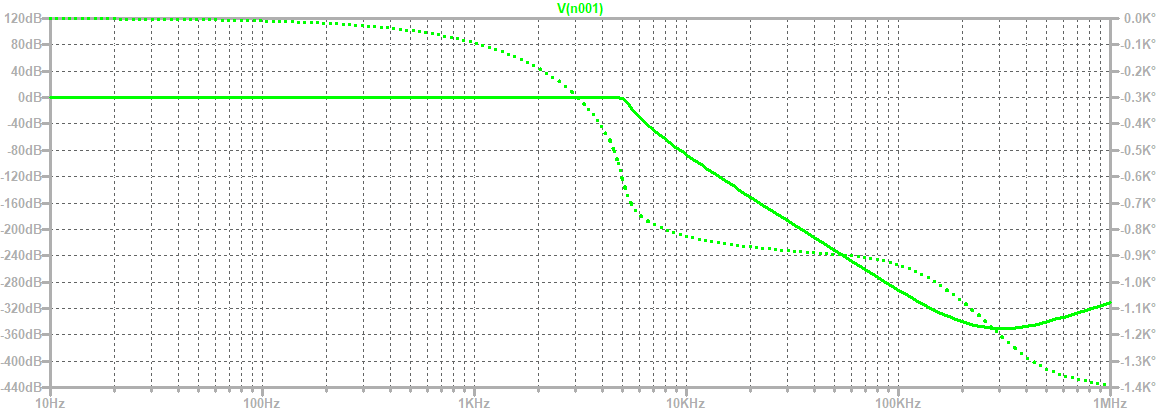
\includegraphics[width=0.8\textwidth]{ImagenesEjercicio2/spice.PNG}
\caption{Respuesta en frecuencia simulada.}
	\label{fig:transspice}
\end{figure}
Luego de esto, se realizó el diseño en altium de la placa a realizar, obteniendo el siguiente diseño:
 \begin{figure}[H]
	\centering
	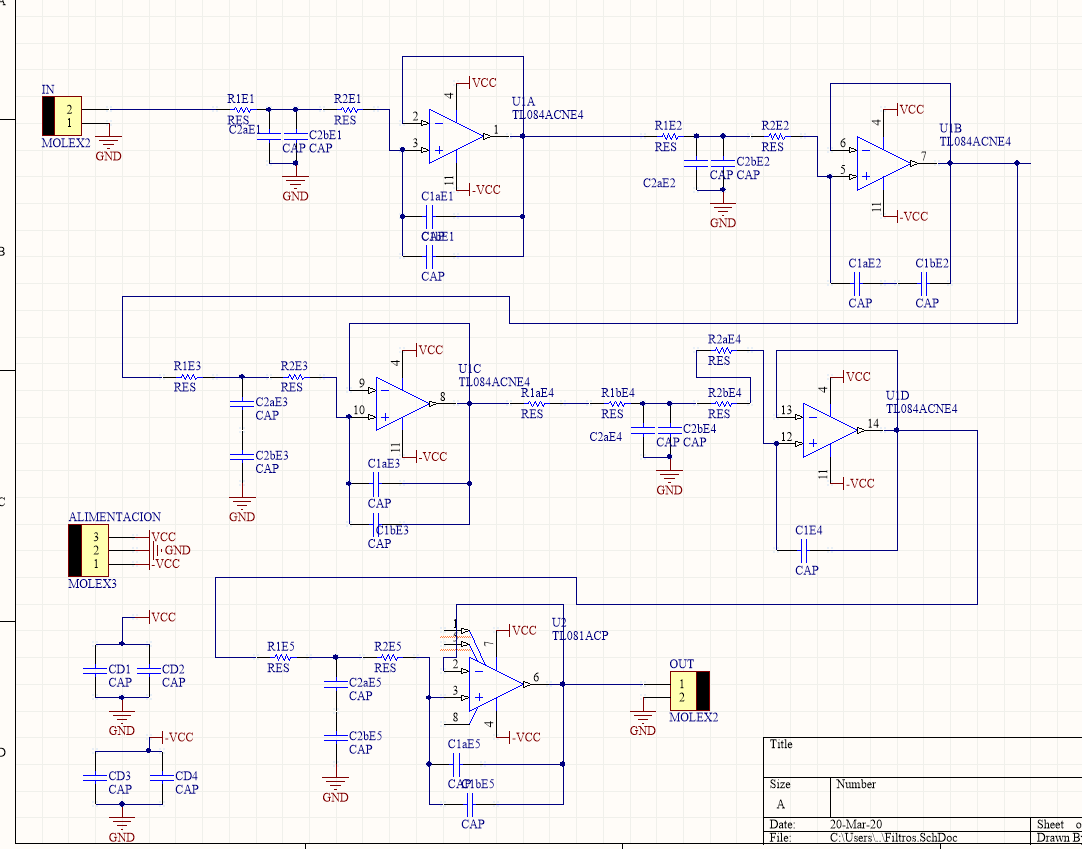
\includegraphics[width=0.8\textwidth]{ImagenesEjercicio2/altiumesq.PNG}
\caption{Esquemático Altium.}
	\label{fig:altiumesq}
\end{figure}
 \begin{figure}[H]
	\centering
	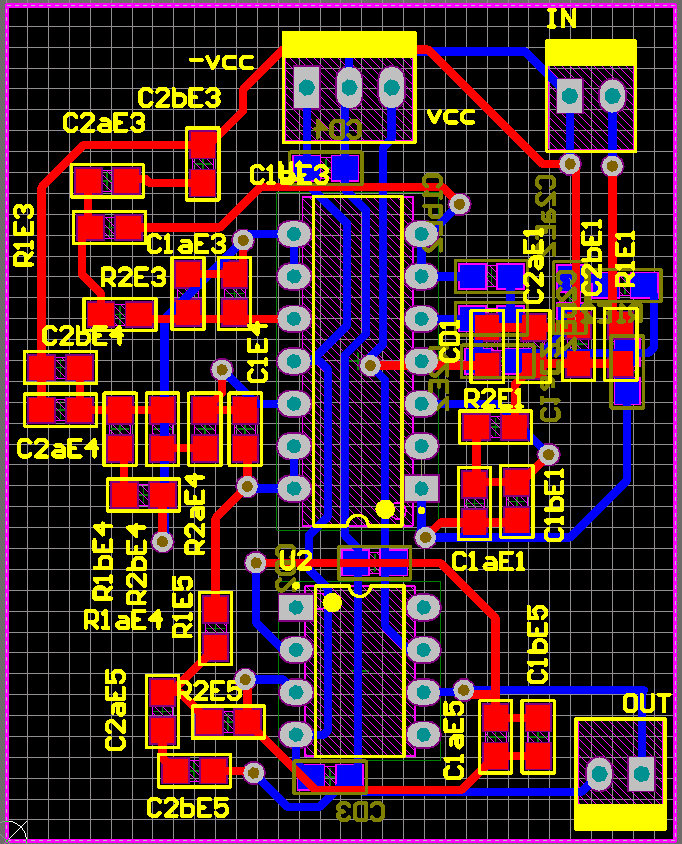
\includegraphics[width=0.8\textwidth]{ImagenesEjercicio2/altiumpcb.PNG}
\caption{PCB Altium.}
	\label{fig:altiumpcb}
\end{figure}
\end{document}